\documentclass[12pt]{article}
%\usepackage[utf8]{inputenc}
%\documentclass[UTF8]{ctexart}
%\usepackage[UTF8, heading = false, scheme = plain]{ctex}
\usepackage{geometry}
%geometry{a4paper,scale=0.9}
\geometry{a4paper,left=1cm,right=1cm,top=1cm,bottom=2cm}
\usepackage{amsfonts}
\usepackage{color}
\usepackage{url}
%\usepackage{biblatex}
\usepackage{amsmath}
\usepackage{amssymb}
\usepackage{latexsym}
\usepackage{cite}
%\addbibresource{ref.bib}
%\bibliography{ref.bib}
\usepackage{caption}
\usepackage{graphicx, subfig}
\usepackage{float}
%\usepackage[fontset=ubuntu]{ctex}
%\usepackage{fontspec}
\usepackage{xeCJK}
%\usepackage[colorlinks,
%anchorcolor=black,
%citecolor=black]{hyperref}
%\setmainfont{SimSun}
\usepackage[section]{placeins}
\usepackage{enumitem}
\usepackage{framed}
\usepackage[framemethod=TikZ]{mdframed}
\usepackage{indentfirst}
\usepackage{setspace}%使用间距宏包
\linespread{1.5}

\title{MAB问题和Bandit算法\cite{Bandit_Algorithm_Recommender_System_Learning_Note}\cite{MAB_And_RL_Introduction}}
\author{leolinuxer}
%\date{June 2020}

\begin{document}
%\setlength{\parindent}{0pt}
\maketitle
\tableofcontents

\section{背景介绍}
推荐系统有两个经典的问题:EE(Exploitation \& Exploration)和冷启动问题。

EE(Exploitation \& Exploration):
\begin{itemize}
\setlength{\itemsep}{0pt}
\setlength{\parsep}{0pt}
\setlength{\parskip}{0pt}
    \item Exploitation:选择现在可能最佳的方案。
    \item Exploration:选择现在不确定的,但未来可能会有高效益的方案
\end{itemize}

比如小红在淘宝上搜索“衣服”,Exploitation 方案呈现的结果都是“衣服”,而Exploration方案呈现的结果可能有“衣服”可能还有搭配的“裤子”、“裙子”。综上:其实EE问题就是涉及到\textbf{准确性和多样性的平衡问题}。我们要怎样在保障准确性的同时增加推荐的多样性呢?针对此问题,Bandit算法可以较好的解决。

\section{MAB问题}
\subsection{MAB问题简介}
Bandit算法来源于历史悠久的赌博学,假想这样的场景:假设面前有$K$台老虎机(arms)。我们知道,老虎机本质上就是个运气游戏,我们假设每台老虎机$i$都有一定概率 $p_i$ 吐出一块钱,或者不吐钱( 概率$1-p_i$)。假设你手上只有 $T$枚代币(tokens),而每摇一次老虎机都需要花费一枚代币,也就是说你一共只能摇$T$次,那么如何做才能使得\textbf{期望回报(expected reward)最大}呢?在这个问题中,如果赌徒一直摇他认为收益最大的老虎机(Exploitation),他就有可能会错过收益更高的老虎机,因此可能还需要进一步探索(Exploration)。这也叫多臂赌博机问题(Multi-armed bandit problem, MAB)。

那么问题的核心是什么呢?自然,我们应该要假设 $p_i$们是不太一样的(不然怎么摇都一样了),即有一些老虎机比较“好”(更容易吐钱),有一些则比较“差”(不太容易吐钱)。

\begin{framed}
理解:

传统的机器学习方法中(实际上也包括其它无监督学习或者半监督学习的很多方法),你并不会动态的去根据收集到的已有的样本去调整你的训练模型,你的训练模型只是单纯被动地获得样本并被教育(instruct,作为对比,active learning主要就是来解决这一问题的)。

而强化学习主要针对的是在一个可能\textbf{不断演化}的环境中,训练一个能\textbf{主动选择自己的动作},并根据动作所返回的不同类型的\textbf{反馈(feedback),动态调整自己接下来的动作},以达到在一个\textbf{比较长期的时间段内平均获得的反馈质量}。因此,在这个问题中,如何evaluate每次获得的反馈,并进行调整,就是RL的核心问题。

将MAB问题对比强化学习的框架,我们的动作是什么?即每次摇哪台老虎机。我们的反馈呢?即我们摇了某台特定的老虎机当回合可以观察它吐了钱没有。
所以,MAB问题广泛应用于 RL 算法中。
\end{framed}


而在推荐系统中,也有很多类似的情景:
\begin{itemize}
\setlength{\itemsep}{0pt}
\setlength{\parsep}{0pt}
\setlength{\parskip}{0pt}
    \item 假设遇到一个新用户,我们不知道他的喜好,该如何推荐他感兴趣的item?或者遇到一个新item,我们不知道怎样的用户会喜欢,该给哪些用户推荐?(即冷启动问题)
    \item 假设我们有若干item,我们应该给用户推荐哪些可以使得效益最大?用户留存率更高?在 保障用户喜好的物品的同时,更加科学的推荐一些新颖的东西提高新颖度?(EE问题)
\end{itemize}

基于此,我们就可以将MAB的思想引入推荐系统。(这感觉就像是:推荐就像一场赌博,老虎机摇出来的是用户满意度+收益,而我们要做一个高智商的赌徒,想办法在一定时间内获得最大的收益,留住更多的用户。)

该如何选择机器呢,这里有个重要的统计学/哲学问题\cite{MAB_And_RL_Introduction}:即我们是\textbf{贝叶斯人(Bayesian)还是频率学家(frequentist)}。对贝叶斯人来说,我们在一进入赌场就对每台老虎机扔钱的概率 $p_i$ 就有一个先验分布(prior distribution)的假设了,比如一个很常见的我们可以用Beta分布。如果我们认为大概率 $p_i$都应该是0.5,即对半开,而不太可能出现一些很极端的情况,我们就可以选择Beta(2,2)分布作为我们的先验分布。然后在我们真正摇了老虎机之后,\textbf{根据相应的反馈},我们就可以\textbf{调整 $p_i$ 们相应的后验分布(posterior distribution)}。比如如果某台机器摇了四五次一直吐不出钱,我们就应该将这台机器的吐钱概率的分布往左推,因为它的 $p_i$大概率应该是小于0.5的。那么,你的任务便是要在有限的时间内找出 $p_i$后验分布比较靠右的那些机器(因为他们更容易吐钱),并且尽可能多的去摇这些比较赚钱的机器。

\begin{figure}[H]
    \centering
    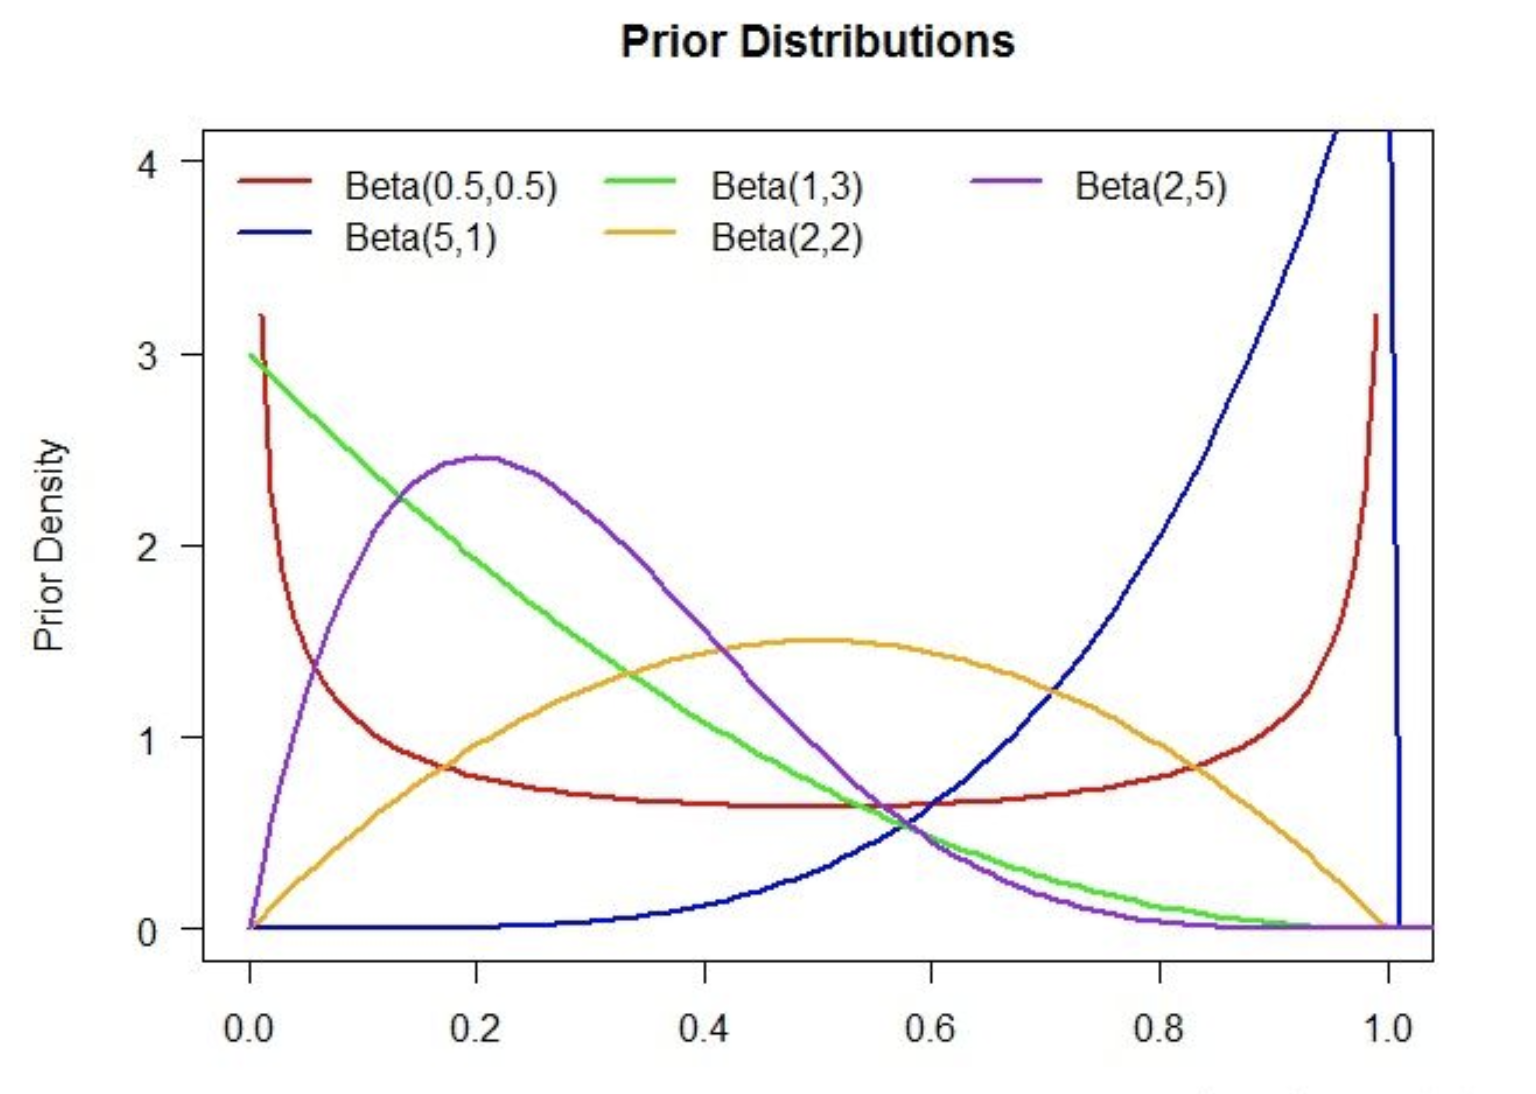
\includegraphics[width=0.6\textwidth]{fig/Bandit-BETA-Examples.png}
\end{figure}

而如果你是频率学家,就没什么先验或者后验分布了,\textbf{你假设你一开始对这些机器的吐钱概率一无所知}。你认为\textbf{每个机器的 $p_i$是个确定的值}。那么,你的任务就是要在有限的时间内找到\textbf{那些高 $p_i$ 的机器,并尽可能多的去摇它们,以获得更多的回报}。那么这里我们注意到这类问题的一大特点,即我们只有 $T$ 次摇机器的机会,如何去平衡这 $T$次中exploration(探索)和exploitation(挖掘)的次数。探索意味着广度,比如如果你是频率学家,你一开始什么都不知道,你至少每个机器都需要稍微摇几次(假设$T > K$ ,不然问题就无法搞定了)才能对每个机器吐钱概率有个大概感觉。然后,你可能会缩小你的搜索范围,再几台机器里重点实验,最后可能就专门摇一台你觉得最容易吐钱的机器了。当然,我们之后会看到这种办法也未必是最好的。

\subsection{MAB问题的变种}
首先,我们前面的讨论默认了环境是不会变化的。而一些MAB问题,这个假设可能不成立,这就好比如果一位玩家发现某个机器的 $p_i$很高,一直摇之后赌场可能人为降低这台机器吐钱的概率。在这种情况下,MAB问题的环境就是随着时间/玩家的行为会发生变化。这类问题,在合理的假设下,也是有不少研究和相应的算法的。目前做的最多的假设,也就是所谓的adversarial bandit(就不是stochastic bandit了),就是说这些 $p_i$ 会被一个“对手”(也可以看成上帝)设定好。如果这是事先设定好,并且在玩家开始有动作之后也无法更改,我们叫做oblivious adversary setting; 如果这个对手在玩家有动作之后还能随时更改自己的设定,那就叫做adaptive adversary setting, 一般要做成zero-sum game了。此外,最近也有一些随机但nonstationary的假设下的工作。

另外MAB有一类很重要的变种,叫做contextual MAB(cMAB)。几乎所有在线广告推送(dynamic ad display)都可以看成是cMAB问题。在这类问题中,每个arm的回报会和当前时段出现的顾客的特征(也就是这里说的context)有关。

另外,如果每台老虎机每天摇的次数有上限,那我们就得到了一个Bandit with Knapsack问题,这类问题以传统组合优化里的背包问题命名,它的研究也和最近不少研究在线背包问题的文章有关,之后我们也会专门讨论。还有很多变种,如Lipshitz bandit, 我们不再有有限台机器,而有无限台(它们的reward function满足利普西茨连续性)等等。


\subsection{MAB问题的样本复杂度(Sample complexity)}
sample complexity是个很有意思的话题。同时,也可以帮助初学者先掌握regret的概念。我们这里仅谈MAB问题的sample complexity, 那么大家也应该会知道这是和RL问题的sample complexity也是密切相关的。Sample complexity, 简单来说,是研究有哪些事情任何bandit算法都是不能做到的。

简单起见,我们只考虑最简单的情形,即我们是频率学家,且环境是stationary的K-arm bandit,也就是说每个arm的reward分布是IID(独立同分布)的,不会随着时间和玩家的行为变化。

凡事都要从最简单开始。我们先令$K=2$ ,即只有两个arms。MAB的样本复杂度,实际上可以看成是这样一个信息论/统计学问题:即,我们有两个Bernouli分布$Ber(p_1), Ber(p_2)$(注意我们假设 $p_1 \neq p_2$),那么我们\textbf{至少}需要分别从这两个分布中获得多少\textbf{样本(samples)},我们才能以\textbf{较大概率}将这两个分布\textbf{区分}开来?

因为实际上只有两个arm,以及MAB问题的特性,实际上,我们只需要能够以较高概率判断出 $p_1$和 $p_2$哪个更大就行了。因为一旦我们能判断出哪个arm的吐钱概率更大,我们自然也就知道了哪个arm更好,我们便自动获得了最优算法(一直摇这个更好的arm就行了)。

而这个问题,不就是说,\textbf{至少要有多少样本,我们才能高置信度地做以下的假设检验}?

$$
If \quad p_1 > p_2
$$

当然到这里还没有结束,有个小技巧便是需要randomization,或者说是计算复杂度理论里最基本的probabilistic method。这个原因也很直观,如果我们构造的例子是确定性的(deterministic),那么必然要么 $p_1 > p_2$或者相反,那么自然在这两种情况下(分别)有两个极其愚蠢的算法都不需要任何样本就能直接“蒙”对,比如前者就是直接猜 $p_1$更大的算法,后者就是直接猜 $p_2$更大的算法。因此,这里的小技巧(trick)就是说我们构造一个随机化(randomized)的例子,比如说在这个例子里0.5的概率 $p_1 > p_2$ ,而0.5的概率 $p_1 < p_2$(你可以想象成我用了两套对arm进行index的方法,这样原来的arm 1就变成了arm 2,原来的arm 2变成了arm 1)。这样的话之前那些愚蠢的算法就至少会有0.5的概率猜错了。而我们的目标就是只要\textbf{证明任何算法都有一定的概率在这个问题上犯错就ok了}!

想明白了以上几点,加上一些KL divergence(最基本的信息论)知识,包括一些什么Pinsker不等式,你就可以证明本节的主要内容了。哦,再让我来介绍下regret的概念。一般来说,我们设计算法的目标就是让期望的regret(一般研究的是regret的upper bound)比较小。那么sample complexity,说的则是相反的一件事情,即无论什么算法,对MAB问题,你\textbf{期望}的regret都\textbf{至少}应该有多大(给的是lower bound)。具体来说,在我们的K-arm例子中,记最大的 $p_i$为$p^*$ ,我们的算法在时刻$t$ 选择的机器是 $i(t)$,那么我们的算法所造成的regret便是:
$$
R(T) = p^* \cdot 1 \cdot T - \sum_{t=1}^Tp_{i(t)} \cdot 1
$$

即,和某个先知相比(一开始就知道 $p^*$),我们所获得的回报和他获得的回报在 $T$ 时间段内的差距。

好了,我们终于可以给出经典的两类lower bound。一类是$\sqrt{T}$的,一类是 $\log{T}$。你可能要说了,$\log{T}$的不是从阶上比$\sqrt{T}$ 更低嘛,那岂不是更紧?而实际上,这两类bound其实可以看成一类,因为前者\textbf{与问题相关的系数无关},而后者有关(我们很快会看到系数具体是什么)。具体为什么这两类bound其实可以看成一类,我在后面介绍UCB算法的时候会再说,感觉在那边会更容易说一些。

注意,这两类lower bound都是有意义的。因为如果你胡乱蒙的话,你的regret至少会随着时间线性增长(即阶为 $\sim T$)。因此,这两类也叫做\textbf{次线性(sublinear)}的regret。

\textbf{定理1}. 对这类MAB问题,存在某一个例子,使得任何的算法都满足
$$
\mathbb{E}[R(T)] \ge \Omega(\sqrt{KT})
$$ 

\textbf{定理2}. 对这类MAB问题,存在某一个例子,使得任何的算法都满足
$$
\mathbb{E}[R(T)] \ge \sum_{a:\Delta(a) > 0} \frac{p^*(1-p^*)}{\Delta(a)}\log{T}
$$

这里$\Delta(a)$ 的定义是$\Delta(a) := p^* - p_a$,即这个arm$a$和最好的arm在期望reward上的差距。这个系数也是我所谓的这类bound实际上里面有跟问题相关的系数。直观理解,虽然$T$的阶比前一类bound要紧了,但是这里乘的系数却更大了。

最后,我们不加说明的点出,贝叶斯版本的K-arm MAB也有相同阶的这两类lower bound。以及,我们确实有算法,可以达到这两类regret,即它们在理论意义上是最优的。


\section{前置知识}
在介绍具体Bandit算法前先补充一个概念:

\subsection{累积遗憾}
赌徒的表现通常用“后悔”来衡量。而最优策略的预期收益(总是拉着最好的手臂)和赌徒的预期收益之间的差距,就是累积遗憾
(regret)。
$$
R_T = \sum_{i=1}^T(w_{opt} - w_{B(i)}) = Tw^* - \sum_{i=1}^Tw_{B(i)}
$$

这里我们讨论的每个臂的收益非0即1,即伯努利收益。每次选择后,计算和最佳的选择的差距,将差距累加起来就是累积遗憾。在上式中, $w_{B(i)}$是第$i$次试验是选中臂的期望收益,而 $w^*$是所有臂中最佳的那个。

这个公式可以用来对比不同Bandit算法的效果:对同样的多臂问题,用不同的Bandit算法试验相同次数,哪个算法的总regret增长最慢,其效果就是比较好的。

\subsection{Beta分布}
有关Beta分布,可以参考帖子:\url{https://www.zhihu.com/question/30269898}。这里只做一个简单的介绍。

beta分布可以看作是一个概率的概率分布。它是对二项分布中成功概率 $p$ 的概率分布的描述。它的形式如下:
$$
Beta(a,b) = \frac{\theta^{a-1}(1-\theta)^{b-1}}{B(a,b)} \propto \theta^{a-1}(1-\theta)^{b-1}
$$

其中,$a$ 和 $b$ 分别代表在 $a+b$ 次伯努利试验中成功和失败的次数。我们用下面的图来说明一下 Beta 分布的含义:
\begin{figure}[H]
    \centering
    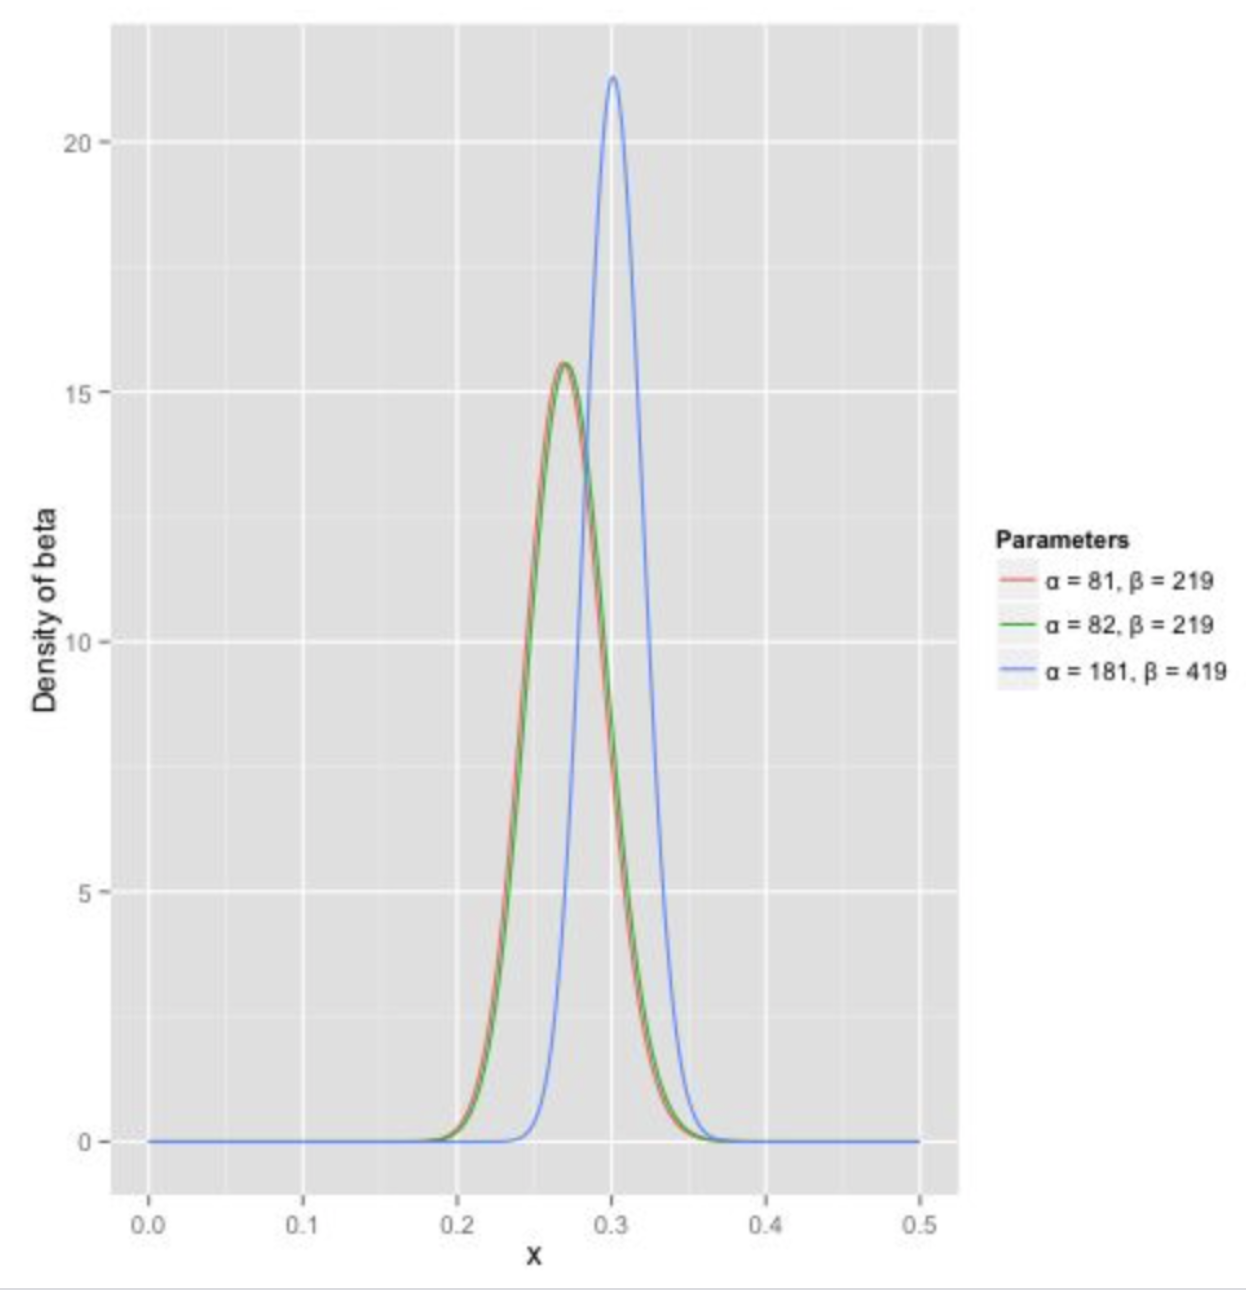
\includegraphics[width=.6\textwidth]{fig/Beta_Example.png}
\end{figure}
上图中一共有三条线,我们忽略中间的一条线,第一条线中 $a=81$,$b=219$。也就是说在我们进行了 300 次伯努利试验中,成功81次,失败219次的情况下,成功概率 $p$ 的一个分布,可以看到,$p$的概率在0.27左右概率最大,但我们不能说成功的概率就是0.27,这也就是频率派和贝叶斯派的区别,哈哈。此时,我们又做了300次试验,此时在总共600次伯努利试验中,成功了181次,失败了419次,此时成功概率 $p$ 的概率分布变为了蓝色的线,在0.3左右概率最大。


\section{Bandit算法}
常见的 Bandit 算法如下:

\subsection{朴素Bandit算法}
先随机试验若干次,计算每个臂的平均收益,一直选均值最大的那个臂。

\subsection{Epsilon-Greedy}
以1-epsilon的概率选取当前收益最大的臂(Exploitation),以epsilon的概率随机选取一个臂(Exploration),即直接用epsilon控制探索(Exploration)的概率,epsilon越接近1,探索的概率越大。
\begin{itemize}
\setlength{\itemsep}{0pt}
\setlength{\parsep}{0pt}
\setlength{\parskip}{0pt}
    \item 优点:简单粗暴
    \item 缺点:探索到一定程度,已经大概知道最优的老虎机了,可能就不需要那么大的epsilon探索了,即epsilon可以变小,更小的成本就可以获得更大的收益。而具体epsilon怎么选取,需要实地去调节。
\end{itemize}

\subsection{Upper Confidence Bound(UCB)}
前面提到了,Epsilon-Greedy算法在探索的时候,所有的老虎机都有同样的概率被选中,这其实没有充分利用历史信息,比如每个老虎机之前探索的次数,每个老虎机之前的探索中吐钱的频率\cite{Recommender_System_With_Deep_Learning_Bandit}。

那我们怎么能够充分利用历史信息呢?首先,根据当前老虎机已经探索的次数,以及吐钱的次数,我们可以计算出当前每个老虎机吐钱的观测概率$p'$。同时,由于观测次数有限,因此观测概率和真实概率 $p$ 之间总会有一定的差值 $ \Delta $ ,即 $p' - \Delta <= p <= p' +  \Delta $。

基于上面的讨论,我们得到了另一种常用的Bandit算法:UCB(Upper Confidence Bound)算法。该算法在每次推荐时,总是乐观的认为每个老虎机能够得到的收益是 $p' +  \Delta $。

好了,接下来的问题就是观测概率和真实概率之间的差值 $ \Delta $ 如何计算了,我们首先有两个直观的理解:

1)对于选中的老虎机,多获得一次反馈会使 $ \Delta $ 变小,当反馈无穷多时,$ \Delta $ 趋近于0,最终会小于其他没有被选中的老虎机的 $ \Delta $。

2)对于没有被选中的老虎机,$ \Delta $ 会随着轮数的增大而增加,最终会大于其他被选中的老虎机。

因此,当进行了一定的轮数的时候,每个老虎机都有机会得到探索的机会。UCB算法中 $p' +  \Delta $的计算公式如下:
$$
p' + \sqrt{\frac{2\ln T}{n}}
$$

其中加号前面是第 $j$ 个老虎机到目前的收益均值,后面的叫做bonus,本质上是均值的标准差,$T$ 是目前的试验次数,$n$ 是该老虎机被试次数。

具体步骤如下:
\begin{enumerate}
\setlength{\itemsep}{0pt}
\setlength{\parsep}{0pt}
\setlength{\parskip}{0pt}
    \item 初始化:先对每个臂都试过一遍
    \item 按照公式计算每个臂的分数,选择分数最大的臂作为选择
    $$
    	\text{UCB}(j) = \bar{x}_j(t) + \sqrt{\frac{2\ln{t}}{T_{j,t}}}
    $$
    \item 观察选择结果,更新$t$和 $T_{j,t}$
\end{enumerate}

其中,$t$为目前试验次数,  $\bar{x}_j(t)$是这个臂到目前的收益均值,$T_{j,t}$ 为这个臂被试次数。$\sqrt{\frac{2\ln{t}}{T_{j,t}}}$就是所谓的置信区间宽度,代表探索的分值。$\bar{x}_j(t) $和 $\sqrt{\frac{2\ln{t}}{T_{j,t}}}$相加就是老虎机 $j$ 的置信区间上界。加号后面本质上就是均值的标准差。

\textcolor{red}{UCB的总体思想其实是:均值越大,标准差越小,被选中的概率会越来越大。}即它总认为探索之后的结果会比现在好,所以除了要选择收益均值最大的臂,还要看它被探索的次数。为了使得每个老虎机被探索的机会次数相当,当某个老虎机的$T_{j,t}$ 越大时(即等式右边的值会越小),给它的机会会越小。

\begin{framed}
理解:

MCTS 算法中根据$UCT$函数选择节点,这里使用$UCB$选择节点;二者本质是一致的;比较如下:
\begin{enumerate}
\setlength{\itemsep}{0pt}
\setlength{\parsep}{0pt}
\setlength{\parskip}{0pt}
    \item \textbf{UCB(Upper Confidence Bound)}
    \item \textbf{UCT(Upper Confidence Bound Apply to Tree)}: UCT = MCTS + UCB,MCTS 表示Monte Carlo tree search
\end{enumerate}

\end{framed}

UCB算法的特点:
\begin{itemize}
\setlength{\itemsep}{0pt}
\setlength{\parsep}{0pt}
\setlength{\parskip}{0pt}
    \item 优点:返回的结果是固定的
    \item 缺点:计算较慢
\end{itemize}

\begin{framed}
\textbf{UCB 公式的由来\cite{Deep_Learning_Recommender_System}}

UCB 公式是基于霍夫丁(Hoeffding Inequality)不等式推导而来的

假设有 $N$ 个范围在 0 到 1 的独立有界随机变量,$X_1, X_2, \cdots, X_n$,那么这 $n$ 个随机变量的经验期望为:
$$
\bar{X} = \frac{X_1 + X_2 + \cdots X_n}{n}
$$

满足下面的霍夫丁不等式:
$$
P(\bar{X} - E[\bar{X}] \ge \varepsilon) \le e^{-2n\varepsilon^2}
$$

接下来,令 
$$
\varepsilon = \sqrt{\frac{2\ln{t}}{T_{j,t}}}
$$

并代入霍夫丁不等式,就有:
$$
P(\bar{X} - E[\bar{X}] \ge \sqrt{\frac{2\ln{t}}{T_{j,t}}}) \le t^{-4}
$$
(霍夫丁不等式中的$n$就是 UCB 中的$T_{j,t}$)

也就是说,如果选择 UCB 的上界是 $\sqrt{\frac{2\ln{t}}{T_{j,t}}}$ 的形式,那么 \textbf{$X$ 的均值与 $X$ 的实际期望的差距在上界之外的概率非常小},小于 $t^{-4}$,这就说明采用 UCB 的上界形式是严格且合理的。

总结来说,就是 \textbf{UCB 的上界形式相当于老虎机收益期望的严格的置信区间}。

~\\

再举个例子(\url{https://www.jianshu.com/p/95b2de50ce44}):

注:这里利用了霍夫丁不等式的另外一个形式,和上面是等价的:
$$
P(\bar{X} - E[\bar{X}] \le \sqrt{\frac{2\ln{t}}{T_{j,t}}}) \ge 1 - \frac{2}{t^{-4}}
$$

当 $\delta$ 取值为 $\sqrt{2\ln T/n}$ 时,可以得到:
$$
P(|\bar(p) - p| \le \sqrt{2\ln T/n} ) \le  
$$

也就是说,$\bar{X} - \sqrt{\frac{2\ln{t}}{T_{j,t}}} \le E[\bar{X}] \le \bar{X} + \sqrt{\frac{2\ln{t}}{T_{j,t}}}$ 是以 $1 - \frac{2}{t^{-4}}$ 的概率成立的:
\begin{itemize}
\setlength{\itemsep}{0pt}
\setlength{\parsep}{0pt}
\setlength{\parskip}{0pt}
    \item 当 $T = 2$ 时,成立的概率为 0.875;
    \item 当 $T = 3$ 时,成立的概率为 0.975;
    \item 当 $T = 4$ 时,成立的概率为 0.992;
\end{itemize}

可以看出 $\Delta = \sqrt{\frac{2\ln{t}}{T_{j,t}}}$ 是一个不错的选择。
\end{framed}

\subsection{Thompson sampling算法}
主要思想是:
\begin{enumerate}
\setlength{\itemsep}{0pt}
\setlength{\parsep}{0pt}
\setlength{\parskip}{0pt}
    \item 假设每个臂能产生收益的概率是$p$,并且$p$的概率分布符合beta(wins, lose);
    \item 每个臂都维护其beta分布的参数,每次试验后,选中一个臂摇一下,有收益的话wins+1,否则,lose+1;
    \item 选择臂的方式则是:通过用每个臂现有的beta分布产生一个随机数,选择所有臂中随机数最大的臂去摇。
\end{enumerate}

算法的特点:
\begin{itemize}
\setlength{\itemsep}{0pt}
\setlength{\parsep}{0pt}
\setlength{\parskip}{0pt}
    \item 优点:实现相对简单,计算量较小
    \item 缺点:返回的结果具有一定随机性,不是确定的事件。
\end{itemize}

\subsection{linUCB方法}
论文(雅虎的新闻推荐算法):\url{https://arxiv.org/pdf/1003.0146.pdf}

解析:\url{https://www.jianshu.com/p/e0e843d78e3c}



\section{扩展阅读}
覃含章:在线学习(MAB)与强化学习(RL)[2]:IID Bandit的一些算法
\url{https://zhuanlan.zhihu.com/p/53595666}

覃含章:在线学习(MAB)与强化学习(RL)[3]:Q learning和UCB算法
\url{https://zhuanlan.zhihu.com/p/54261100}

覃含章:在线学习(MAB)与强化学习(RL)[4]:贝叶斯Bandit算法
\url{https://zhuanlan.zhihu.com/p/55254900}

覃含章:在线学习(MAB)与强化学习(RL)[5]:贝叶斯RL算法
\url{https://zhuanlan.zhihu.com/p/55578013}


%\printbibliography
\bibliography{../ref}
\bibliographystyle{IEEEtran}
\end{document}